\section{Introduction}
\label{sec:introduction}
Realising flexible industrial automation systems requires an approach
 for autonomous and distributed designs \cite{Lyu.2021}. Programmable Logic Controllers (PLCs) are the established platform for real-time control software that accesses sensors and actuators \cite{Sehr.2021}.  Standards play an important role in distributed automation, for instance, IEC~61131-3 and IEC~61499, which define programming paradigms for control software development \cite{Lyu.2021}. %Despite the increasing complexity of automation systems, the programming models of IEC 61131-3 are still prevalent \cite{Sehr.2021}. 
 Multiple interacting PLCs form a distributed control system. Providing the respective engineering methodologies and models is a goal of IEC~61499 \cite{61499}. Heterogeneous systems can even be composed of PLCs from various vendors and programmed with different tools \cite{lyu2020towards} \cite{mazzolini2017structured}. Furthermore, a single development tool can distribute control code across multiple runtime environments (RTEs)~\cite{eclipse4diac}, motivating the need to execute component tests in each of these RTEs. Developers of IEC~61499 library modules  \cite{oberlehner.2022} will also need to provide their modules to users of various development environments. 
 Despite the focus on portability \cite{61499} and the standardized XML format for data exchange \cite{61499.2}, IEC~61499-based software components must often be modified during the porting process \cite{Hopsu.2019, Testing_Midhun}. Due to varying execution behaviour, the ported software may behave differently on each platform \cite{Testing_Midhun, Wiesmayr.2023}, possibly leading to malfunctions of the distributed control system. Therefore, it is crucial to thoroughly test an IEC 61499 application on each relevant target platform before using the software in a real-world system. A platform-independent test specification has the potential to greatly reduce the involved effort.
\begin{figure*}[t]
    \centering
    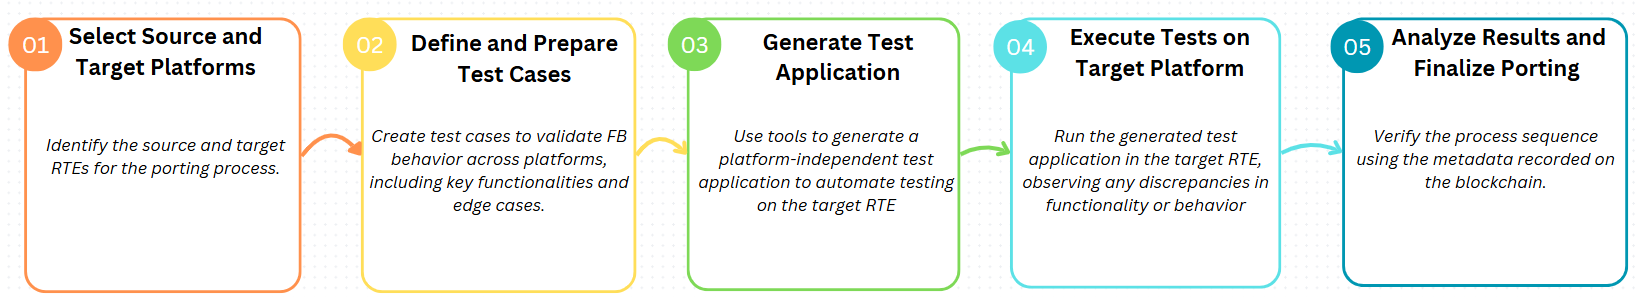
\includegraphics[width=0.95\linewidth]{OJIES_2024/Figures/portingProcessPNG.PNG}
    \caption{Process of porting test code for IEC~61499 Function Blocks between execution environments.}
    \label{fig:porting_process}
\end{figure*}
%The IEC 61499 standard \cite{61499} addresses the issues of vendor lock-in and offers a solution by providing a framework for developing portable and interoperable software. Although the file exchange format is standardised, it is currently interpreted differently and the execution behavior varies among vendors \cite{christensen.2012,Thramboulidis.2009}. 

%\todo[inline]{MX: add references and details, paragraph is complicated to read}
Evaluating a system's correctness typically involves providing test data and observing the system's reaction. Such tests are specified manually, obtained from models, or generated using other techniques \cite{Sinha.2019}. The engineering processes of complex control systems additionally require that PLC platforms ensure reliability through simulation and verification, rather than relying on iterative testing of a cyber-physical system \cite{Sehr.2021}. Simulation methods evaluate only a system model and, thus, can provide results faster \cite{Sinha.2019}. In the context of IEC~61499, executing test cases within a run-time environment can be considered a simulation. A certain degree of test automation is required to efficiently evaluate this software. Existing test processes for IEC~61499-based software rely on a framework in the target platform (e.g., \cite{hametner2014}) and are therefore not applicable for cross-platform development of IEC~61499-based software. When (re-)using parts of IEC~61499 software in multiple platforms, extensions to the IEC~61499 standard may not be available in all platforms (equally). Hence, we are investigating an approach for test automation that does not require any extensions of IEC~61499.

% Current control systems are highly dependent on specific vendors, hindering the transfer of programs between different platforms \cite{}. As seamless integration is a key requirement in the context of Industry 4.0, this lack of portability poses great challenges \cite{}.

%As a result, migrating programs from one IEC 61499 platform to another, and thus executing them in a different run-time environment (RTE), may introduce errors that are difficult to detect but could lead to damage to humans or the physical equipment \cite{Testing_Midhun}. Therefore, it is crucial to thoroughly test an IEC 61499 application on the target platform before deploying it to a real-world system. A platform-independent test specification has the potential to greatly reduce the involved effort.
\begin{rquestion}{Research Question (RQ)}
    How can we automate the testing of IEC 61499 software components to evaluate their correct behaviour across platforms from different vendors?
\end{rquestion}

This paper aims to address the challenge of evaluating the effect of porting software components to other platforms or configuring additional RTEs. The test framework allows us to execute tests in any IEC~61499-compliant RTE. Based on our initial concept presented in \cite{biancaMidhunETFAwip}, we generate an IEC~61499-compliant test application that automatically provides test events and data, compares the results of the software component under test with the expected observable behaviour and summarises the results so that they are accessible by the user. The general process is visualised in Figure~\ref{fig:porting_process}. 
Like Hametner et al.~\cite{hametner2014}, we use service sequence models as test specifications. Related work in the context of testing and porting IEC~61499 components is outlined in Section~\ref{sec::sota}. Section~\ref{sec::running_example} introduces a running example. Based on this example, Section~\ref{sec::methodology} outlines the envisioned methodology to test FBs on any IEC~61499-compliant platform. 
One of these IDEs, the 4diac IDE from the Eclipse 4diac open source project, was extended to generate the test application. 
The generation rules for a test application and their implementation are described in Section~\ref{sec::implementation}. Realised as a composite FB, the test application is portable across various IEC 61499 platforms and enables validation of the correct functionality before deployment in real-world machinery. We evaluated our approach using a demonstrator (Section~\ref{sec::casestudy}). Section~\ref{sec::results} lists the identified portability issues and programming errors that we could detect using our test suite. In addition, we discuss limitations of our approach before concluding our paper in Section~\ref{sec::conclusions}. 


%Previous work showed the feasibility of using service sequences as test specifications \cite{wiesmayr2021,hametner2014}. 
%Existing testing mechanisms require dedicated tool support and cannot be directly transferred to other platforms. The portability of IEC 61499 software allows migrating applications to other IEC 61499 vendor platforms, but ensuring that a program behaves consistently across RTEs remains an open challenge. 
%In this paper, we therefore present our approach for testing FBs that allows to execute tests on any IEC 61499-compliant RTE. Based on test scenarios that are created as a service sequence model, we generate the corresponding test application. %FB, establish the necessary connections with the FB under test, execute each test scenario, compare the results, and provide the test outcome. 